5. $\cfrac{(x^2-1)(2x^2-5x-7)}{2-x}\leqslant0\Leftrightarrow\cfrac{(x-1)(x+1)^2\cdot 2\left(x-\cfrac{7}{2}
ight)}{2-x}\leqslant0.$ Применив метод интервалов, найдём ответ:
\begin{figure}[ht!]
\center{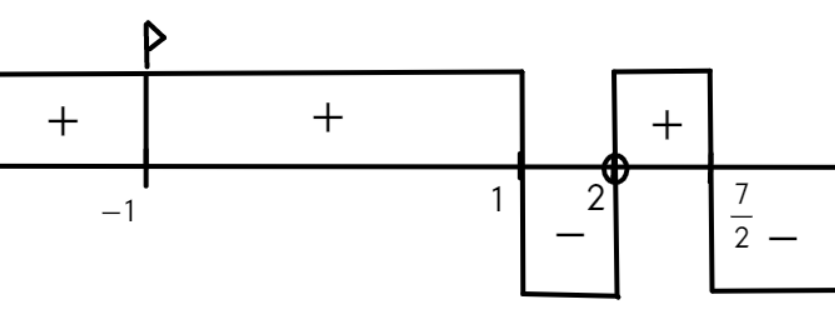
\includegraphics[scale=0.35]{int5.png}}
\end{figure}
$x\in\{-1\}\cup[1;2)\cup\left[\cfrac{7}{2};+\infty
ight).$\\
